% Created by tikzDevice version 0.12
% !TEX encoding = UTF-8 Unicode
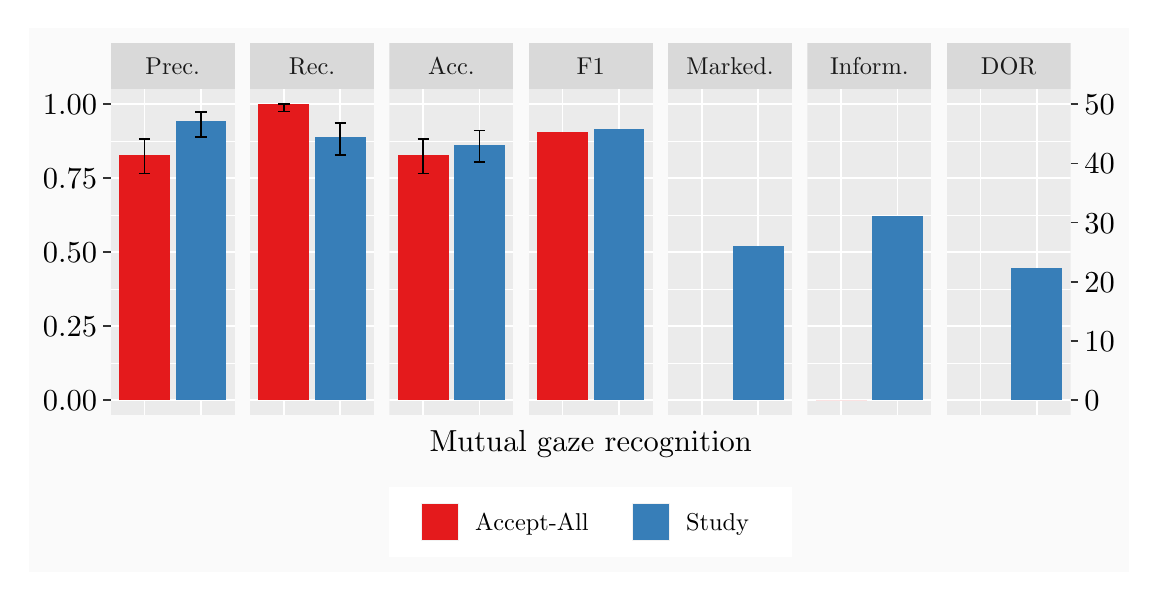
\begin{tikzpicture}[x=1pt,y=1pt]
\definecolor{fillColor}{RGB}{255,255,255}
\path[use as bounding box,fill=fillColor,fill opacity=0.00] (0,0) rectangle (398.34,196.94);
\begin{scope}
\path[clip] (  0.00,  0.00) rectangle (398.34,196.94);
\definecolor{drawColor}{RGB}{255,255,255}
\definecolor{fillColor}{gray}{0.98}

\path[draw=drawColor,line width= 0.6pt,line join=round,line cap=round,fill=fillColor] (  0.00,  0.00) rectangle (398.34,196.94);
\end{scope}
\begin{scope}
\path[clip] ( 30.00, 56.97) rectangle ( 74.84,174.63);
\definecolor{fillColor}{gray}{0.92}

\path[fill=fillColor] ( 30.00, 56.97) rectangle ( 74.84,174.63);
\definecolor{drawColor}{RGB}{255,255,255}

\path[draw=drawColor,line width= 0.3pt,line join=round] ( 30.00, 75.69) --
	( 74.84, 75.69);

\path[draw=drawColor,line width= 0.3pt,line join=round] ( 30.00,102.43) --
	( 74.84,102.43);

\path[draw=drawColor,line width= 0.3pt,line join=round] ( 30.00,129.17) --
	( 74.84,129.17);

\path[draw=drawColor,line width= 0.3pt,line join=round] ( 30.00,155.92) --
	( 74.84,155.92);

\path[draw=drawColor,line width= 0.6pt,line join=round] ( 30.00, 62.32) --
	( 74.84, 62.32);

\path[draw=drawColor,line width= 0.6pt,line join=round] ( 30.00, 89.06) --
	( 74.84, 89.06);

\path[draw=drawColor,line width= 0.6pt,line join=round] ( 30.00,115.80) --
	( 74.84,115.80);

\path[draw=drawColor,line width= 0.6pt,line join=round] ( 30.00,142.54) --
	( 74.84,142.54);

\path[draw=drawColor,line width= 0.6pt,line join=round] ( 30.00,169.29) --
	( 74.84,169.29);

\path[draw=drawColor,line width= 0.6pt,line join=round] ( 42.23, 56.97) --
	( 42.23,174.63);

\path[draw=drawColor,line width= 0.6pt,line join=round] ( 62.61, 56.97) --
	( 62.61,174.63);
\definecolor{fillColor}{RGB}{228,26,28}

\path[fill=fillColor] ( 33.06, 62.32) rectangle ( 51.40,151.05);
\definecolor{fillColor}{RGB}{55,126,184}

\path[fill=fillColor] ( 53.44, 62.32) rectangle ( 71.78,163.08);
\definecolor{drawColor}{RGB}{0,0,0}

\path[draw=drawColor,line width= 0.6pt,line join=round] ( 60.57,166.57) --
	( 64.65,166.57);

\path[draw=drawColor,line width= 0.6pt,line join=round] ( 62.61,166.57) --
	( 62.61,157.41);

\path[draw=drawColor,line width= 0.6pt,line join=round] ( 60.57,157.41) --
	( 64.65,157.41);

\path[draw=drawColor,line width= 0.6pt,line join=round] ( 40.19,156.66) --
	( 44.27,156.66);

\path[draw=drawColor,line width= 0.6pt,line join=round] ( 42.23,156.66) --
	( 42.23,144.22);

\path[draw=drawColor,line width= 0.6pt,line join=round] ( 40.19,144.22) --
	( 44.27,144.22);
\end{scope}
\begin{scope}
\path[clip] ( 80.34, 56.97) rectangle (125.18,174.63);
\definecolor{fillColor}{gray}{0.92}

\path[fill=fillColor] ( 80.34, 56.97) rectangle (125.18,174.63);
\definecolor{drawColor}{RGB}{255,255,255}

\path[draw=drawColor,line width= 0.3pt,line join=round] ( 80.34, 75.69) --
	(125.18, 75.69);

\path[draw=drawColor,line width= 0.3pt,line join=round] ( 80.34,102.43) --
	(125.18,102.43);

\path[draw=drawColor,line width= 0.3pt,line join=round] ( 80.34,129.17) --
	(125.18,129.17);

\path[draw=drawColor,line width= 0.3pt,line join=round] ( 80.34,155.92) --
	(125.18,155.92);

\path[draw=drawColor,line width= 0.6pt,line join=round] ( 80.34, 62.32) --
	(125.18, 62.32);

\path[draw=drawColor,line width= 0.6pt,line join=round] ( 80.34, 89.06) --
	(125.18, 89.06);

\path[draw=drawColor,line width= 0.6pt,line join=round] ( 80.34,115.80) --
	(125.18,115.80);

\path[draw=drawColor,line width= 0.6pt,line join=round] ( 80.34,142.54) --
	(125.18,142.54);

\path[draw=drawColor,line width= 0.6pt,line join=round] ( 80.34,169.29) --
	(125.18,169.29);

\path[draw=drawColor,line width= 0.6pt,line join=round] ( 92.57, 56.97) --
	( 92.57,174.63);

\path[draw=drawColor,line width= 0.6pt,line join=round] (112.95, 56.97) --
	(112.95,174.63);
\definecolor{fillColor}{RGB}{228,26,28}

\path[fill=fillColor] ( 83.40, 62.32) rectangle (101.74,169.29);
\definecolor{fillColor}{RGB}{55,126,184}

\path[fill=fillColor] (103.78, 62.32) rectangle (122.13,157.56);
\definecolor{drawColor}{RGB}{0,0,0}

\path[draw=drawColor,line width= 0.6pt,line join=round] (110.92,162.45) --
	(114.99,162.45);

\path[draw=drawColor,line width= 0.6pt,line join=round] (112.95,162.45) --
	(112.95,150.90);

\path[draw=drawColor,line width= 0.6pt,line join=round] (110.92,150.90) --
	(114.99,150.90);

\path[draw=drawColor,line width= 0.6pt,line join=round] ( 90.53,169.29) --
	( 94.61,169.29);

\path[draw=drawColor,line width= 0.6pt,line join=round] ( 92.57,169.29) --
	( 92.57,166.62);

\path[draw=drawColor,line width= 0.6pt,line join=round] ( 90.53,166.62) --
	( 94.61,166.62);
\end{scope}
\begin{scope}
\path[clip] (130.68, 56.97) rectangle (175.53,174.63);
\definecolor{fillColor}{gray}{0.92}

\path[fill=fillColor] (130.68, 56.97) rectangle (175.53,174.63);
\definecolor{drawColor}{RGB}{255,255,255}

\path[draw=drawColor,line width= 0.3pt,line join=round] (130.68, 75.69) --
	(175.53, 75.69);

\path[draw=drawColor,line width= 0.3pt,line join=round] (130.68,102.43) --
	(175.53,102.43);

\path[draw=drawColor,line width= 0.3pt,line join=round] (130.68,129.17) --
	(175.53,129.17);

\path[draw=drawColor,line width= 0.3pt,line join=round] (130.68,155.92) --
	(175.53,155.92);

\path[draw=drawColor,line width= 0.6pt,line join=round] (130.68, 62.32) --
	(175.53, 62.32);

\path[draw=drawColor,line width= 0.6pt,line join=round] (130.68, 89.06) --
	(175.53, 89.06);

\path[draw=drawColor,line width= 0.6pt,line join=round] (130.68,115.80) --
	(175.53,115.80);

\path[draw=drawColor,line width= 0.6pt,line join=round] (130.68,142.54) --
	(175.53,142.54);

\path[draw=drawColor,line width= 0.6pt,line join=round] (130.68,169.29) --
	(175.53,169.29);

\path[draw=drawColor,line width= 0.6pt,line join=round] (142.91, 56.97) --
	(142.91,174.63);

\path[draw=drawColor,line width= 0.6pt,line join=round] (163.30, 56.97) --
	(163.30,174.63);
\definecolor{fillColor}{RGB}{228,26,28}

\path[fill=fillColor] (133.74, 62.32) rectangle (152.09,151.05);
\definecolor{fillColor}{RGB}{55,126,184}

\path[fill=fillColor] (154.12, 62.32) rectangle (172.47,154.70);
\definecolor{drawColor}{RGB}{0,0,0}

\path[draw=drawColor,line width= 0.6pt,line join=round] (161.26,159.73) --
	(165.33,159.73);

\path[draw=drawColor,line width= 0.6pt,line join=round] (163.30,159.73) --
	(163.30,148.31);

\path[draw=drawColor,line width= 0.6pt,line join=round] (161.26,148.31) --
	(165.33,148.31);

\path[draw=drawColor,line width= 0.6pt,line join=round] (140.88,156.66) --
	(144.95,156.66);

\path[draw=drawColor,line width= 0.6pt,line join=round] (142.91,156.66) --
	(142.91,144.22);

\path[draw=drawColor,line width= 0.6pt,line join=round] (140.88,144.22) --
	(144.95,144.22);
\end{scope}
\begin{scope}
\path[clip] (181.03, 56.97) rectangle (225.87,174.63);
\definecolor{fillColor}{gray}{0.92}

\path[fill=fillColor] (181.03, 56.97) rectangle (225.87,174.63);
\definecolor{drawColor}{RGB}{255,255,255}

\path[draw=drawColor,line width= 0.3pt,line join=round] (181.03, 75.69) --
	(225.87, 75.69);

\path[draw=drawColor,line width= 0.3pt,line join=round] (181.03,102.43) --
	(225.87,102.43);

\path[draw=drawColor,line width= 0.3pt,line join=round] (181.03,129.17) --
	(225.87,129.17);

\path[draw=drawColor,line width= 0.3pt,line join=round] (181.03,155.92) --
	(225.87,155.92);

\path[draw=drawColor,line width= 0.6pt,line join=round] (181.03, 62.32) --
	(225.87, 62.32);

\path[draw=drawColor,line width= 0.6pt,line join=round] (181.03, 89.06) --
	(225.87, 89.06);

\path[draw=drawColor,line width= 0.6pt,line join=round] (181.03,115.80) --
	(225.87,115.80);

\path[draw=drawColor,line width= 0.6pt,line join=round] (181.03,142.54) --
	(225.87,142.54);

\path[draw=drawColor,line width= 0.6pt,line join=round] (181.03,169.29) --
	(225.87,169.29);

\path[draw=drawColor,line width= 0.6pt,line join=round] (193.25, 56.97) --
	(193.25,174.63);

\path[draw=drawColor,line width= 0.6pt,line join=round] (213.64, 56.97) --
	(213.64,174.63);
\definecolor{fillColor}{RGB}{228,26,28}

\path[fill=fillColor] (184.08, 62.32) rectangle (202.43,159.32);
\definecolor{fillColor}{RGB}{55,126,184}

\path[fill=fillColor] (204.47, 62.32) rectangle (222.81,160.25);
\end{scope}
\begin{scope}
\path[clip] (231.37, 56.97) rectangle (276.21,174.63);
\definecolor{fillColor}{gray}{0.92}

\path[fill=fillColor] (231.37, 56.97) rectangle (276.21,174.63);
\definecolor{drawColor}{RGB}{255,255,255}

\path[draw=drawColor,line width= 0.3pt,line join=round] (231.37, 75.69) --
	(276.21, 75.69);

\path[draw=drawColor,line width= 0.3pt,line join=round] (231.37,102.43) --
	(276.21,102.43);

\path[draw=drawColor,line width= 0.3pt,line join=round] (231.37,129.17) --
	(276.21,129.17);

\path[draw=drawColor,line width= 0.3pt,line join=round] (231.37,155.92) --
	(276.21,155.92);

\path[draw=drawColor,line width= 0.6pt,line join=round] (231.37, 62.32) --
	(276.21, 62.32);

\path[draw=drawColor,line width= 0.6pt,line join=round] (231.37, 89.06) --
	(276.21, 89.06);

\path[draw=drawColor,line width= 0.6pt,line join=round] (231.37,115.80) --
	(276.21,115.80);

\path[draw=drawColor,line width= 0.6pt,line join=round] (231.37,142.54) --
	(276.21,142.54);

\path[draw=drawColor,line width= 0.6pt,line join=round] (231.37,169.29) --
	(276.21,169.29);

\path[draw=drawColor,line width= 0.6pt,line join=round] (243.60, 56.97) --
	(243.60,174.63);

\path[draw=drawColor,line width= 0.6pt,line join=round] (263.98, 56.97) --
	(263.98,174.63);
\definecolor{fillColor}{RGB}{55,126,184}

\path[fill=fillColor] (254.81, 62.32) rectangle (273.15,118.05);
\end{scope}
\begin{scope}
\path[clip] (281.71, 56.97) rectangle (326.55,174.63);
\definecolor{fillColor}{gray}{0.92}

\path[fill=fillColor] (281.71, 56.97) rectangle (326.55,174.63);
\definecolor{drawColor}{RGB}{255,255,255}

\path[draw=drawColor,line width= 0.3pt,line join=round] (281.71, 75.69) --
	(326.55, 75.69);

\path[draw=drawColor,line width= 0.3pt,line join=round] (281.71,102.43) --
	(326.55,102.43);

\path[draw=drawColor,line width= 0.3pt,line join=round] (281.71,129.17) --
	(326.55,129.17);

\path[draw=drawColor,line width= 0.3pt,line join=round] (281.71,155.92) --
	(326.55,155.92);

\path[draw=drawColor,line width= 0.6pt,line join=round] (281.71, 62.32) --
	(326.55, 62.32);

\path[draw=drawColor,line width= 0.6pt,line join=round] (281.71, 89.06) --
	(326.55, 89.06);

\path[draw=drawColor,line width= 0.6pt,line join=round] (281.71,115.80) --
	(326.55,115.80);

\path[draw=drawColor,line width= 0.6pt,line join=round] (281.71,142.54) --
	(326.55,142.54);

\path[draw=drawColor,line width= 0.6pt,line join=round] (281.71,169.29) --
	(326.55,169.29);

\path[draw=drawColor,line width= 0.6pt,line join=round] (293.94, 56.97) --
	(293.94,174.63);

\path[draw=drawColor,line width= 0.6pt,line join=round] (314.32, 56.97) --
	(314.32,174.63);
\definecolor{fillColor}{RGB}{228,26,28}

\path[fill=fillColor] (284.77, 62.32) rectangle (303.11, 62.32);
\definecolor{fillColor}{RGB}{55,126,184}

\path[fill=fillColor] (305.15, 62.32) rectangle (323.49,129.04);
\end{scope}
\begin{scope}
\path[clip] (332.05, 56.97) rectangle (376.89,174.63);
\definecolor{fillColor}{gray}{0.92}

\path[fill=fillColor] (332.05, 56.97) rectangle (376.89,174.63);
\definecolor{drawColor}{RGB}{255,255,255}

\path[draw=drawColor,line width= 0.3pt,line join=round] (332.05, 75.69) --
	(376.89, 75.69);

\path[draw=drawColor,line width= 0.3pt,line join=round] (332.05,102.43) --
	(376.89,102.43);

\path[draw=drawColor,line width= 0.3pt,line join=round] (332.05,129.17) --
	(376.89,129.17);

\path[draw=drawColor,line width= 0.3pt,line join=round] (332.05,155.92) --
	(376.89,155.92);

\path[draw=drawColor,line width= 0.6pt,line join=round] (332.05, 62.32) --
	(376.89, 62.32);

\path[draw=drawColor,line width= 0.6pt,line join=round] (332.05, 89.06) --
	(376.89, 89.06);

\path[draw=drawColor,line width= 0.6pt,line join=round] (332.05,115.80) --
	(376.89,115.80);

\path[draw=drawColor,line width= 0.6pt,line join=round] (332.05,142.54) --
	(376.89,142.54);

\path[draw=drawColor,line width= 0.6pt,line join=round] (332.05,169.29) --
	(376.89,169.29);

\path[draw=drawColor,line width= 0.6pt,line join=round] (344.28, 56.97) --
	(344.28,174.63);

\path[draw=drawColor,line width= 0.6pt,line join=round] (364.66, 56.97) --
	(364.66,174.63);
\definecolor{fillColor}{RGB}{55,126,184}

\path[fill=fillColor] (355.49, 62.32) rectangle (373.83,110.12);
\end{scope}
\begin{scope}
\path[clip] ( 30.00,174.63) rectangle ( 74.84,191.44);
\definecolor{fillColor}{gray}{0.85}

\path[fill=fillColor] ( 30.00,174.63) rectangle ( 74.84,191.44);
\definecolor{drawColor}{gray}{0.10}

\node[text=drawColor,anchor=base,inner sep=0pt, outer sep=0pt, scale=  0.88] at ( 52.42,180.01) {Prec.};
\end{scope}
\begin{scope}
\path[clip] ( 80.34,174.63) rectangle (125.18,191.44);
\definecolor{fillColor}{gray}{0.85}

\path[fill=fillColor] ( 80.34,174.63) rectangle (125.18,191.44);
\definecolor{drawColor}{gray}{0.10}

\node[text=drawColor,anchor=base,inner sep=0pt, outer sep=0pt, scale=  0.88] at (102.76,180.01) {Rec.};
\end{scope}
\begin{scope}
\path[clip] (130.68,174.63) rectangle (175.53,191.44);
\definecolor{fillColor}{gray}{0.85}

\path[fill=fillColor] (130.68,174.63) rectangle (175.53,191.44);
\definecolor{drawColor}{gray}{0.10}

\node[text=drawColor,anchor=base,inner sep=0pt, outer sep=0pt, scale=  0.88] at (153.10,180.01) {Acc.};
\end{scope}
\begin{scope}
\path[clip] (181.03,174.63) rectangle (225.87,191.44);
\definecolor{fillColor}{gray}{0.85}

\path[fill=fillColor] (181.03,174.63) rectangle (225.87,191.44);
\definecolor{drawColor}{gray}{0.10}

\node[text=drawColor,anchor=base,inner sep=0pt, outer sep=0pt, scale=  0.88] at (203.45,180.01) {F1};
\end{scope}
\begin{scope}
\path[clip] (231.37,174.63) rectangle (276.21,191.44);
\definecolor{fillColor}{gray}{0.85}

\path[fill=fillColor] (231.37,174.63) rectangle (276.21,191.44);
\definecolor{drawColor}{gray}{0.10}

\node[text=drawColor,anchor=base,inner sep=0pt, outer sep=0pt, scale=  0.88] at (253.79,180.01) {Marked.};
\end{scope}
\begin{scope}
\path[clip] (281.71,174.63) rectangle (326.55,191.44);
\definecolor{fillColor}{gray}{0.85}

\path[fill=fillColor] (281.71,174.63) rectangle (326.55,191.44);
\definecolor{drawColor}{gray}{0.10}

\node[text=drawColor,anchor=base,inner sep=0pt, outer sep=0pt, scale=  0.88] at (304.13,180.01) {Inform.};
\end{scope}
\begin{scope}
\path[clip] (332.05,174.63) rectangle (376.89,191.44);
\definecolor{fillColor}{gray}{0.85}

\path[fill=fillColor] (332.05,174.63) rectangle (376.89,191.44);
\definecolor{drawColor}{gray}{0.10}

\node[text=drawColor,anchor=base,inner sep=0pt, outer sep=0pt, scale=  0.88] at (354.47,180.01) {DOR};
\end{scope}
\begin{scope}
\path[clip] (  0.00,  0.00) rectangle (398.34,196.94);
\definecolor{drawColor}{RGB}{0,0,0}

\node[text=drawColor,anchor=base east,inner sep=0pt, outer sep=0pt, scale=  1.10] at ( 25.05, 58.53) {0.00};

\node[text=drawColor,anchor=base east,inner sep=0pt, outer sep=0pt, scale=  1.10] at ( 25.05, 85.28) {0.25};

\node[text=drawColor,anchor=base east,inner sep=0pt, outer sep=0pt, scale=  1.10] at ( 25.05,112.02) {0.50};

\node[text=drawColor,anchor=base east,inner sep=0pt, outer sep=0pt, scale=  1.10] at ( 25.05,138.76) {0.75};

\node[text=drawColor,anchor=base east,inner sep=0pt, outer sep=0pt, scale=  1.10] at ( 25.05,165.50) {1.00};
\end{scope}
\begin{scope}
\path[clip] (  0.00,  0.00) rectangle (398.34,196.94);
\definecolor{drawColor}{gray}{0.20}

\path[draw=drawColor,line width= 0.6pt,line join=round] ( 27.25, 62.32) --
	( 30.00, 62.32);

\path[draw=drawColor,line width= 0.6pt,line join=round] ( 27.25, 89.06) --
	( 30.00, 89.06);

\path[draw=drawColor,line width= 0.6pt,line join=round] ( 27.25,115.80) --
	( 30.00,115.80);

\path[draw=drawColor,line width= 0.6pt,line join=round] ( 27.25,142.54) --
	( 30.00,142.54);

\path[draw=drawColor,line width= 0.6pt,line join=round] ( 27.25,169.29) --
	( 30.00,169.29);
\end{scope}
\begin{scope}
\path[clip] (  0.00,  0.00) rectangle (398.34,196.94);
\definecolor{drawColor}{gray}{0.20}

\path[draw=drawColor,line width= 0.6pt,line join=round] (376.89, 62.32) --
	(379.64, 62.32);

\path[draw=drawColor,line width= 0.6pt,line join=round] (376.89, 83.71) --
	(379.64, 83.71);

\path[draw=drawColor,line width= 0.6pt,line join=round] (376.89,105.11) --
	(379.64,105.11);

\path[draw=drawColor,line width= 0.6pt,line join=round] (376.89,126.50) --
	(379.64,126.50);

\path[draw=drawColor,line width= 0.6pt,line join=round] (376.89,147.89) --
	(379.64,147.89);

\path[draw=drawColor,line width= 0.6pt,line join=round] (376.89,169.29) --
	(379.64,169.29);
\end{scope}
\begin{scope}
\path[clip] (  0.00,  0.00) rectangle (398.34,196.94);
\definecolor{drawColor}{RGB}{0,0,0}

\node[text=drawColor,anchor=base west,inner sep=0pt, outer sep=0pt, scale=  1.10] at (381.84, 58.53) {0};

\node[text=drawColor,anchor=base west,inner sep=0pt, outer sep=0pt, scale=  1.10] at (381.84, 79.93) {10};

\node[text=drawColor,anchor=base west,inner sep=0pt, outer sep=0pt, scale=  1.10] at (381.84,101.32) {20};

\node[text=drawColor,anchor=base west,inner sep=0pt, outer sep=0pt, scale=  1.10] at (381.84,122.71) {30};

\node[text=drawColor,anchor=base west,inner sep=0pt, outer sep=0pt, scale=  1.10] at (381.84,144.10) {40};

\node[text=drawColor,anchor=base west,inner sep=0pt, outer sep=0pt, scale=  1.10] at (381.84,165.50) {50};
\end{scope}
\begin{scope}
\path[clip] (  0.00,  0.00) rectangle (398.34,196.94);
\definecolor{drawColor}{RGB}{0,0,0}

\node[text=drawColor,anchor=base,inner sep=0pt, outer sep=0pt, scale=  1.10] at (203.45, 43.90) {Mutual gaze recognition};
\end{scope}
\begin{scope}
\path[clip] (  0.00,  0.00) rectangle (398.34,196.94);
\definecolor{fillColor}{RGB}{255,255,255}

\path[fill=fillColor] (130.72,  5.50) rectangle (276.17, 30.95);
\end{scope}
\begin{scope}
\path[clip] (  0.00,  0.00) rectangle (398.34,196.94);
\definecolor{drawColor}{RGB}{255,255,255}
\definecolor{fillColor}{gray}{0.95}

\path[draw=drawColor,line width= 0.6pt,line join=round,line cap=round,fill=fillColor] (141.72, 11.00) rectangle (156.18, 25.45);
\end{scope}
\begin{scope}
\path[clip] (  0.00,  0.00) rectangle (398.34,196.94);
\definecolor{fillColor}{RGB}{228,26,28}

\path[fill=fillColor] (142.43, 11.71) rectangle (155.46, 24.74);
\end{scope}
\begin{scope}
\path[clip] (  0.00,  0.00) rectangle (398.34,196.94);
\definecolor{drawColor}{RGB}{255,255,255}
\definecolor{fillColor}{gray}{0.95}

\path[draw=drawColor,line width= 0.6pt,line join=round,line cap=round,fill=fillColor] (217.99, 11.00) rectangle (232.44, 25.45);
\end{scope}
\begin{scope}
\path[clip] (  0.00,  0.00) rectangle (398.34,196.94);
\definecolor{fillColor}{RGB}{55,126,184}

\path[fill=fillColor] (218.70, 11.71) rectangle (231.73, 24.74);
\end{scope}
\begin{scope}
\path[clip] (  0.00,  0.00) rectangle (398.34,196.94);
\definecolor{drawColor}{RGB}{0,0,0}

\node[text=drawColor,anchor=base west,inner sep=0pt, outer sep=0pt, scale=  0.88] at (161.68, 15.20) {Accept-All};
\end{scope}
\begin{scope}
\path[clip] (  0.00,  0.00) rectangle (398.34,196.94);
\definecolor{drawColor}{RGB}{0,0,0}

\node[text=drawColor,anchor=base west,inner sep=0pt, outer sep=0pt, scale=  0.88] at (237.94, 15.20) {Study};
\end{scope}
\end{tikzpicture}
